\section{Concepts and Principles}
\label{sec:principles}

%\label{sec:supervised}
The goal of Supervised Machine Learning can be summarized in one sentence:
Estimate a model based on some data, and then use the model to predict the
expected outcome for some new cases, for which we do not know the outcome yet.
Which is exactly what we have done in the introductory example in Section~\ref{sec:prediction}.

But when do we need it?

In short, in any scenario where the following two preconditions are fulfilled.
First, we have a large dataset (say, $100,000$
headlines) for which we want to predict to which class they belong (say, whether
they are clickbait or not).
Second, for a random subset of the data (say, $2,000$ of the headlines), we already
know the class.
For example because we have manually coded (``annotated'') them.

Before we start using SML, though, we first need to have
a common terminology.
At the risk of oversimplifying matters, Table~\ref{tab:mllingo} provides a rough
guideline of how some typical machine learning terms translate to statistical
terms that you may be familiar with.

\begin{table}
\caption{Some common machine learning terms explained\label{tab:mllingo}}{
  \centering
\begin{tabularx}{\textwidth}{XX}
\toprule
machine learning lingo  & statistics lingo\\ \midrule
feature                 & independent variable  \\
label                   & dependent variable  \\
labeled dataset         & dataset with both independent and dependent variables\\
to train a model        & to estimate \\
classifier (classification)  & model to predict nominal outcomes \\
to annotate             & to (manually) code (content analysis) \\
\bottomrule
\end{tabularx}}{}
\end{table}

Let us explain them more in detail by walking through a typical SML workflow.

Before we start, we need to get a \emph{labeled dataset}.
It may be given to us, or we need to create it ourselves.
For instance, often we can draw a random sample of our data and use techniques
of manual content analysis \citep[e.g.,][]{riffe2019analyzing} to
\emph{annotate} (i.e., to manually code) the data.
You can download an example for this process (annotating the topic of news
articles) from \url{http://dx.doi.org/10.6084/m9.figshare.7314896.v1} \citep{Vermeer2018}.

It is hard to give a rule of thumb of how many labelled data you need.
It depends heavily on the type of data you have (if it is a \emph{binary} or a \emph{multi-class} classification problem), and on how evenly distributed (\emph{class balance}) they are (after all, having $10,000$ annotated headlines doesn't help you if $9,990$ are no clickbait and only $10$ are).
These reservations notwithstanding, it is fair to say that typical sizes in
our field are (very roughly) speaking often in the order of $1,000$ to $10,000$
when classifying longer texts \citep[see]{Burscher2014},
even though researchers studying less rich data sometimes annotate larger
datasets \citep[e.g., $60,000$ social media messages in][]{vermeer2019seeing}.

Once we have established that this labelled dataset is available and
have ensured that it is of good quality, we randomly split it into two
datasets: a \emph{training dataset} and a \emph{test
  dataset}.\footnote{In Section~\ref{sec:validation}, we discuss more
  advanced approaches, such as splitting into training, validation,
  and test dataset, and cross-validation.}  We will use the first one
to train our model, and the second to test how good our model
performs. Common ratios range from 50:50 to 80:20; and especially if
the size of your labelled dataset is rather limited, you may want to
have a slightly larger training dataset at the expense of a slightly
smaller test dataset.

In \refex{preparedata}, we prepare the dataset we already used in
Section~\ref{sec:prediction} for classification by creating a
dichotomous variable (the label) and splitting it into a training and
a test dataset. We use |y_train| to denote the training labels and
|X_train| to denote the feature matrix of the training dataset;
|y_test| and |X_test| is the corresponding test dataset. We set a
so-called random-state seed to make sure that the random splitting
will be the same when re-running the code. We can easily split these datasets using the \pkg{rsample} function \fn{initial\_split} in R and the \pkg{sklearn} function \fn{train\_test\_split} in Python.

\pyrex[output=py, caption=Preparing a dataset for supervised machine learning]{chapter09/preparedata}

We now can \emph{train our classifier} (i.e., estimate our model using the
training dataset contained in the objects \texttt{X\_train} and \texttt{y\_train}). This can be as straightforward as estimating a
logistic regression equation (we will discuss different classifiers in
Section~\ref{sec:nb2dnn}).  It may be that we first need to create new
independent variables, so-called features, a step known as
\emph{feature engineering}, for example by transforming existing
variables, combining them, or by converting text numerical word
frequencies.
\refex{nb} shows how easy it is to train a classifier using the Na\"ive Bayes algorithm with packages \pkg{caret}/\pkg{naivebayes} in R and \pkg{sklearn} in Python (this approach will be better explained in Subsection~\ref{subsec:Na\"ive Bayes}).

\pyrex[output=none, caption=A simple Na\"ive Bayes classifier]{chapter09/nb}

But before we can actually use this classifier to do some useful work,
though, we need to test how capable it actually is to predict the
correct labels, given a set of features. One might think that we could
just feed it the same input data (i.e., the same features) again and
see whether the predicted labels match the actual labels of the test
dataset.  In fact, we could do that.  But this test would not be
strict enough: After all, the classifier has been trained on exactly
these data, and therefore one would expect it to perform pretty well.
In particular, it may be that the classifier is very good in
predicting its own training data, but fails at predicting other data,
because it overgeneralizes some idiosyncrasy in the data, a phenomenon
known as overfitting (see Figure ~\ref{fig:roccurve}).

\begin{figure} 
\centering
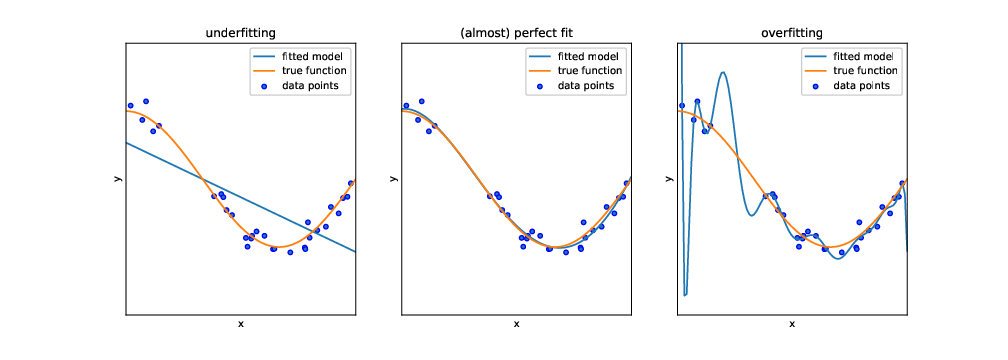
\includegraphics[width=\linewidth]{figures/ch09_overfitting}
\caption{Underfitting and overfitting. Example adapted from https://scikit-learn.org/stable/auto\_examples/model\_selection/plot\_underfitting\_overfitting.html}
\label{fig:roccurve}
\end{figure}

Instead, we use the features of the \emph{test dataset} (stored in the objects  \texttt{X\_test} and \texttt{y\_test})  as input for
our classifier, and evaluate in how far the predicted labels match the
actual labels.  Remember: the classifier has at no point in time seen
the actual labels.  Therefore, we can in fact calculate how often the
prediction is right\footnote{We assume here that the manual annotation
  is always right; an assumption that one may, of course,
  challenge. However, in the absence of any better proxy for reality,
  we assume that this manual annotation is the so-called \emph{gold
    standard} that reflects the \emph{ground truth} as closely as
  possible, and that by definition cannot be outperformed. The manual annotation might has some reliability measures to ensure its quality, such as the \emph{intercoder reliability} which tests the degree of agreement between two or more annotators in order to check if our classes are well defined and the coders are doing their work correctly.}

\pyrex[output=py, caption=Calculating precision and recall]{chapter09/classificationreport}

As shown in \refex{classificationreport}, we can create a \emph{confusion matrix} (generated with \pkg{caret} function \fn{confusionMatrix} in R and \pkg{sklearn} function \fn{confusion\_matrix} in Python), and then estimate two measures: \emph{precision} and \emph{recall} (using base R calculations in R and \pkg{sklearn} function \fn{classification\_report} in Python). In a binary classification, the \emph{confusion matrix} is a useful table in which each column usually represents the number of cases in a predicted class, and each row the number of cases in the real or actual class. With this matrix we can then estimate the number of \emph{true positives} (TP) (correct prediction), \emph{false positives} (FP) (incorrect prediction), \emph{true negatives} (TN) (correct prediction) and \emph{false negatives} (FN) (incorrect prediction).

For a better understanding of these concepts, imagine now that we build a sentiment classifier, that predicts -- based on the
text of a movie review -- whether it is a positive review or a
negative review. Let us assume that the goal of training this classifier is to build an app that recommends the user only good movies. There are two things
that we want to achieve: We want to find as many as possible positive
films (recall), but we also want that the selection we found
\emph{only} contains positive films (precision).

Precision is calculated as $\frac{TP}{TP+FP}$, where TP are true
positives and FP are false positives. For example, if our classifier
retrieves 200 articles that it classifies as positive films, but only
150 of them indeed are positive films, then the precision is
$\frac{150}{150+50} = \frac{150}{200} = 0.75$.

Recall is calculated as $\frac{TP}{TP+FN}$, where TP are true
positives and FN are false negatives. If we know that the classifier
from the previous paragraph missed 20 positive films, then the recall
is $\frac{150}{150+20} = \frac{150}{170}= 0.88$.

In other words: Recall measures how many of the cases we wanted to
find we actually found. Precision measures how much of what we have
found actually is correct.

Often, we have to make a trade-off between precision and recall. For
example, just retrieving \emph{every} film would give us a recall of
1.0 (after all, we didn't miss a single positive film). But on the
other hand, we retrieved all the negative films as well, so precision
will be extremely low. It can depend on the task at hand whether
precision or recall is more important. In
Section~\ref{sec:validation}, we discuss this tradeoff in detail, as well as other metrics such as \emph{accuracy}, \emph{f1-score} or the \emph{area under the curve} (AUC).
